\subsection{Metodologías ágiles}
Las metodologías ágiles son un conjunto de metodologías de desarrollo de software
que se caracterizan por ser iterativas e incrementales. Estas metodologías se
basan en el desarrollo de software en ciclos cortos de tiempo, llamados
iteraciones, en los que se desarrolla una parte del software. Estas iteraciones
son incrementales, es decir, cada iteración añade una funcionalidad al software
que se está desarrollando. De esta forma, se consigue que el software se
desarrolle de forma incremental, y que se pueda ir probando y testeando a medida
que se desarrolla. Esto permite que se puedan detectar errores de forma temprana
y que se puedan corregir de forma rápida. Además, permite que el software se
pueda adaptar a los cambios que se produzcan en los requisitos del proyecto.\medskip

A diferencia de las metodologías tradicionales o pesadas \cite{Jose_1634898355000} 
(como por ejemplo el modelo en cascada), las metodologías ágiles no se basan en la planificación
inicial del proyecto, sino que se basan en la adaptación constante, cualidad
que es muy importante especialmente en proyectos de investigación, en los que
la planificación inicial es muy difícil de realizar debido a la incertidumbre
que existe en este tipo de proyectos y a los diversos factores externos que
pueden afectar al proyecto.

\begin{figure}[ht]
    \centering
    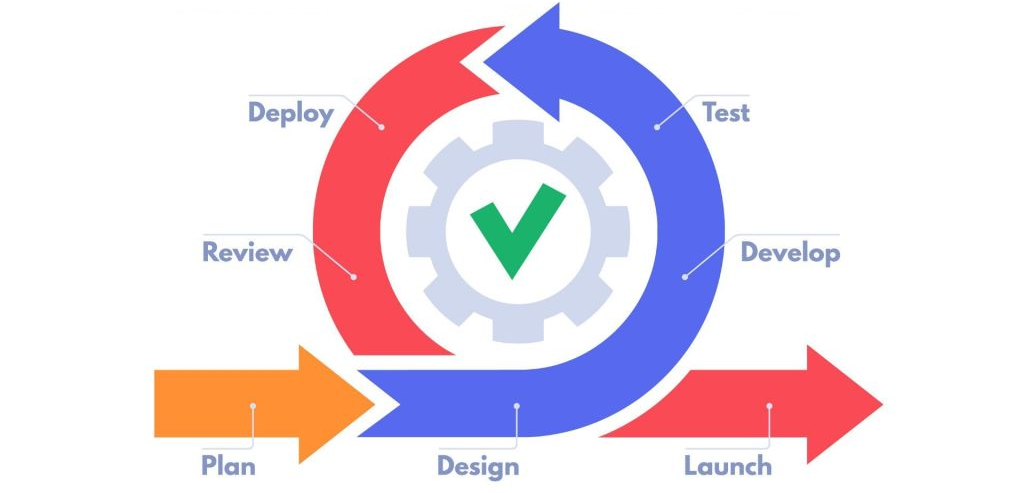
\includegraphics[width=\textwidth]{agile.png}
    \caption{Flujo de trabajo de una metodología ágil.}
    \label{fig:agile}
\end{figure}
